\section{Performance Evaluation}
\label{sec:performance-eval}

The experiments were evaluated with PyTorch which runs on a six-core Ubuntu 18.04 and 16GB of RAM.
ShieldFL was evaluated on the MNIST \cite{deng2012mnist} and KDDCup99 \cite{tavallaee2009detailed} datasets.
To prove that the proposed scheme is generic, the former is an example of an image-based dataset, while the latter is an example of a text-based dataset.
\Cref{fig:acc-comparison} presents accuracy comparison between ShieldFL and state-of-the-art schemes.
It is clear that in non-IID settings, ShieldFL surpasses all other schemes with an average overall accuracy of $90\%$.
However, it is slightly lower than [13] in IID settings.
Overall, we can say that ShieldFL has a fixed high accuracy in both IID and non-IDD settings.
It is worth mentioning that the reference numbers are taken from the original paper \cite{ma2022shieldfl}.

\begin{figure}[thb]
\centering
  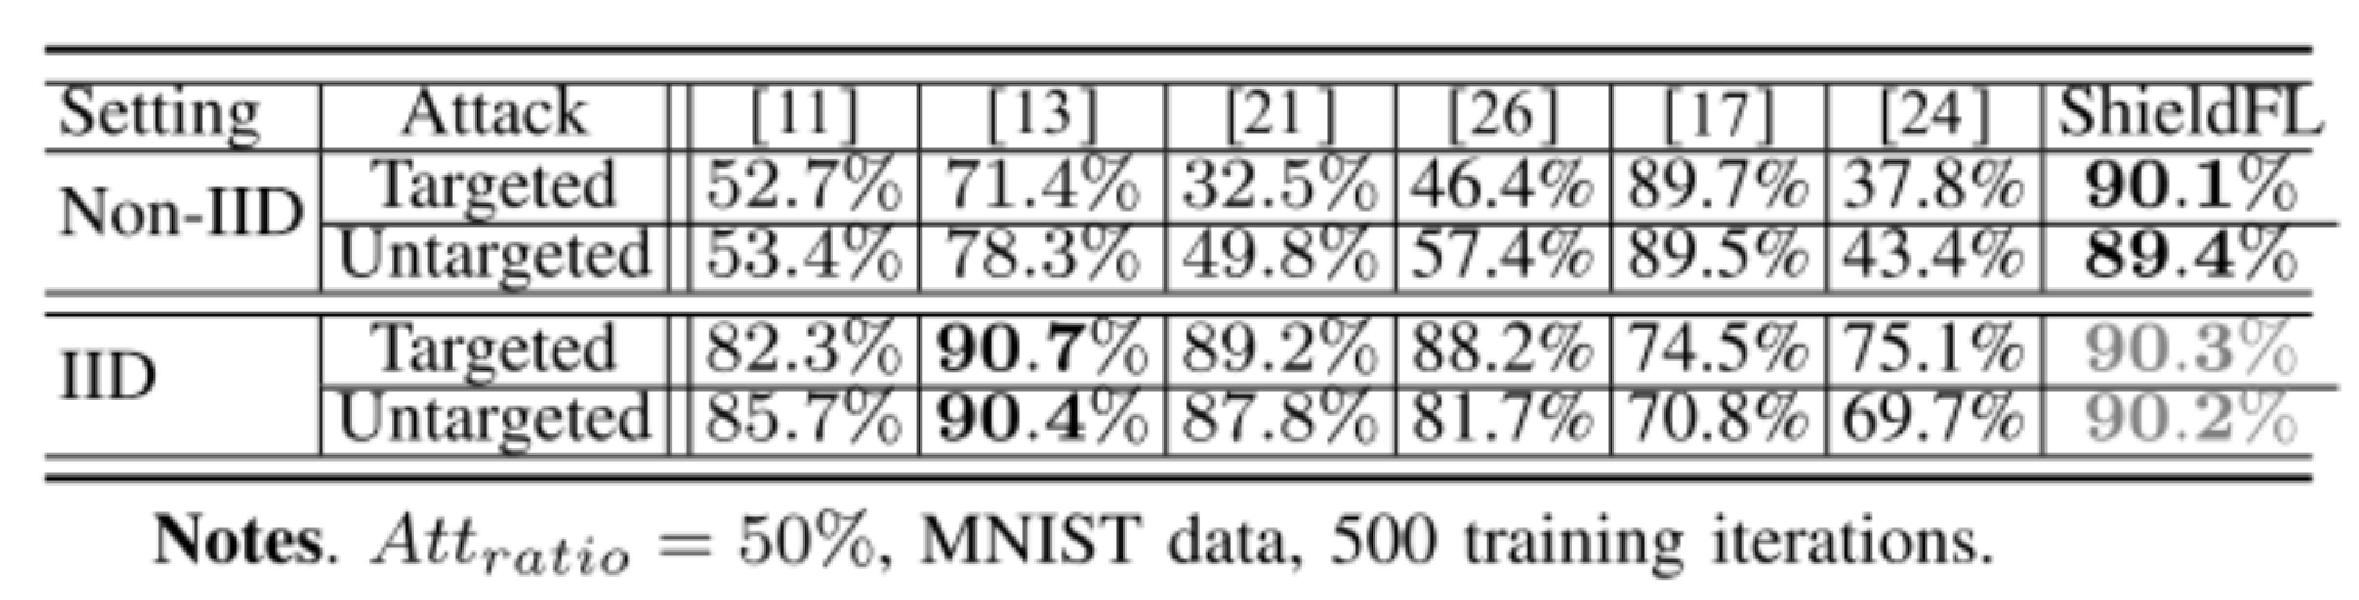
\includegraphics[width=0.8\linewidth]{resources/accuracy-comparison-table.pdf}
  \caption{Accuracy comparison between ShieldFL and existing schemes}
  \label{fig:acc-comparison}
  %\vspace{-5mm}
\end{figure}

\Cref{fig:mnsist-accuracy-comparison} compares the schemes in the non-IID setting when the ratio of malicious users is $50\%$.
The graph on the left shows a targeted attack scenario where the malicious users target a specific label, while the graph on the right depicts an untargeted attack scenario where the malicious users want to degrade the accuracy of the system regardless of the label.

\begin{figure}[thb]
\centering
  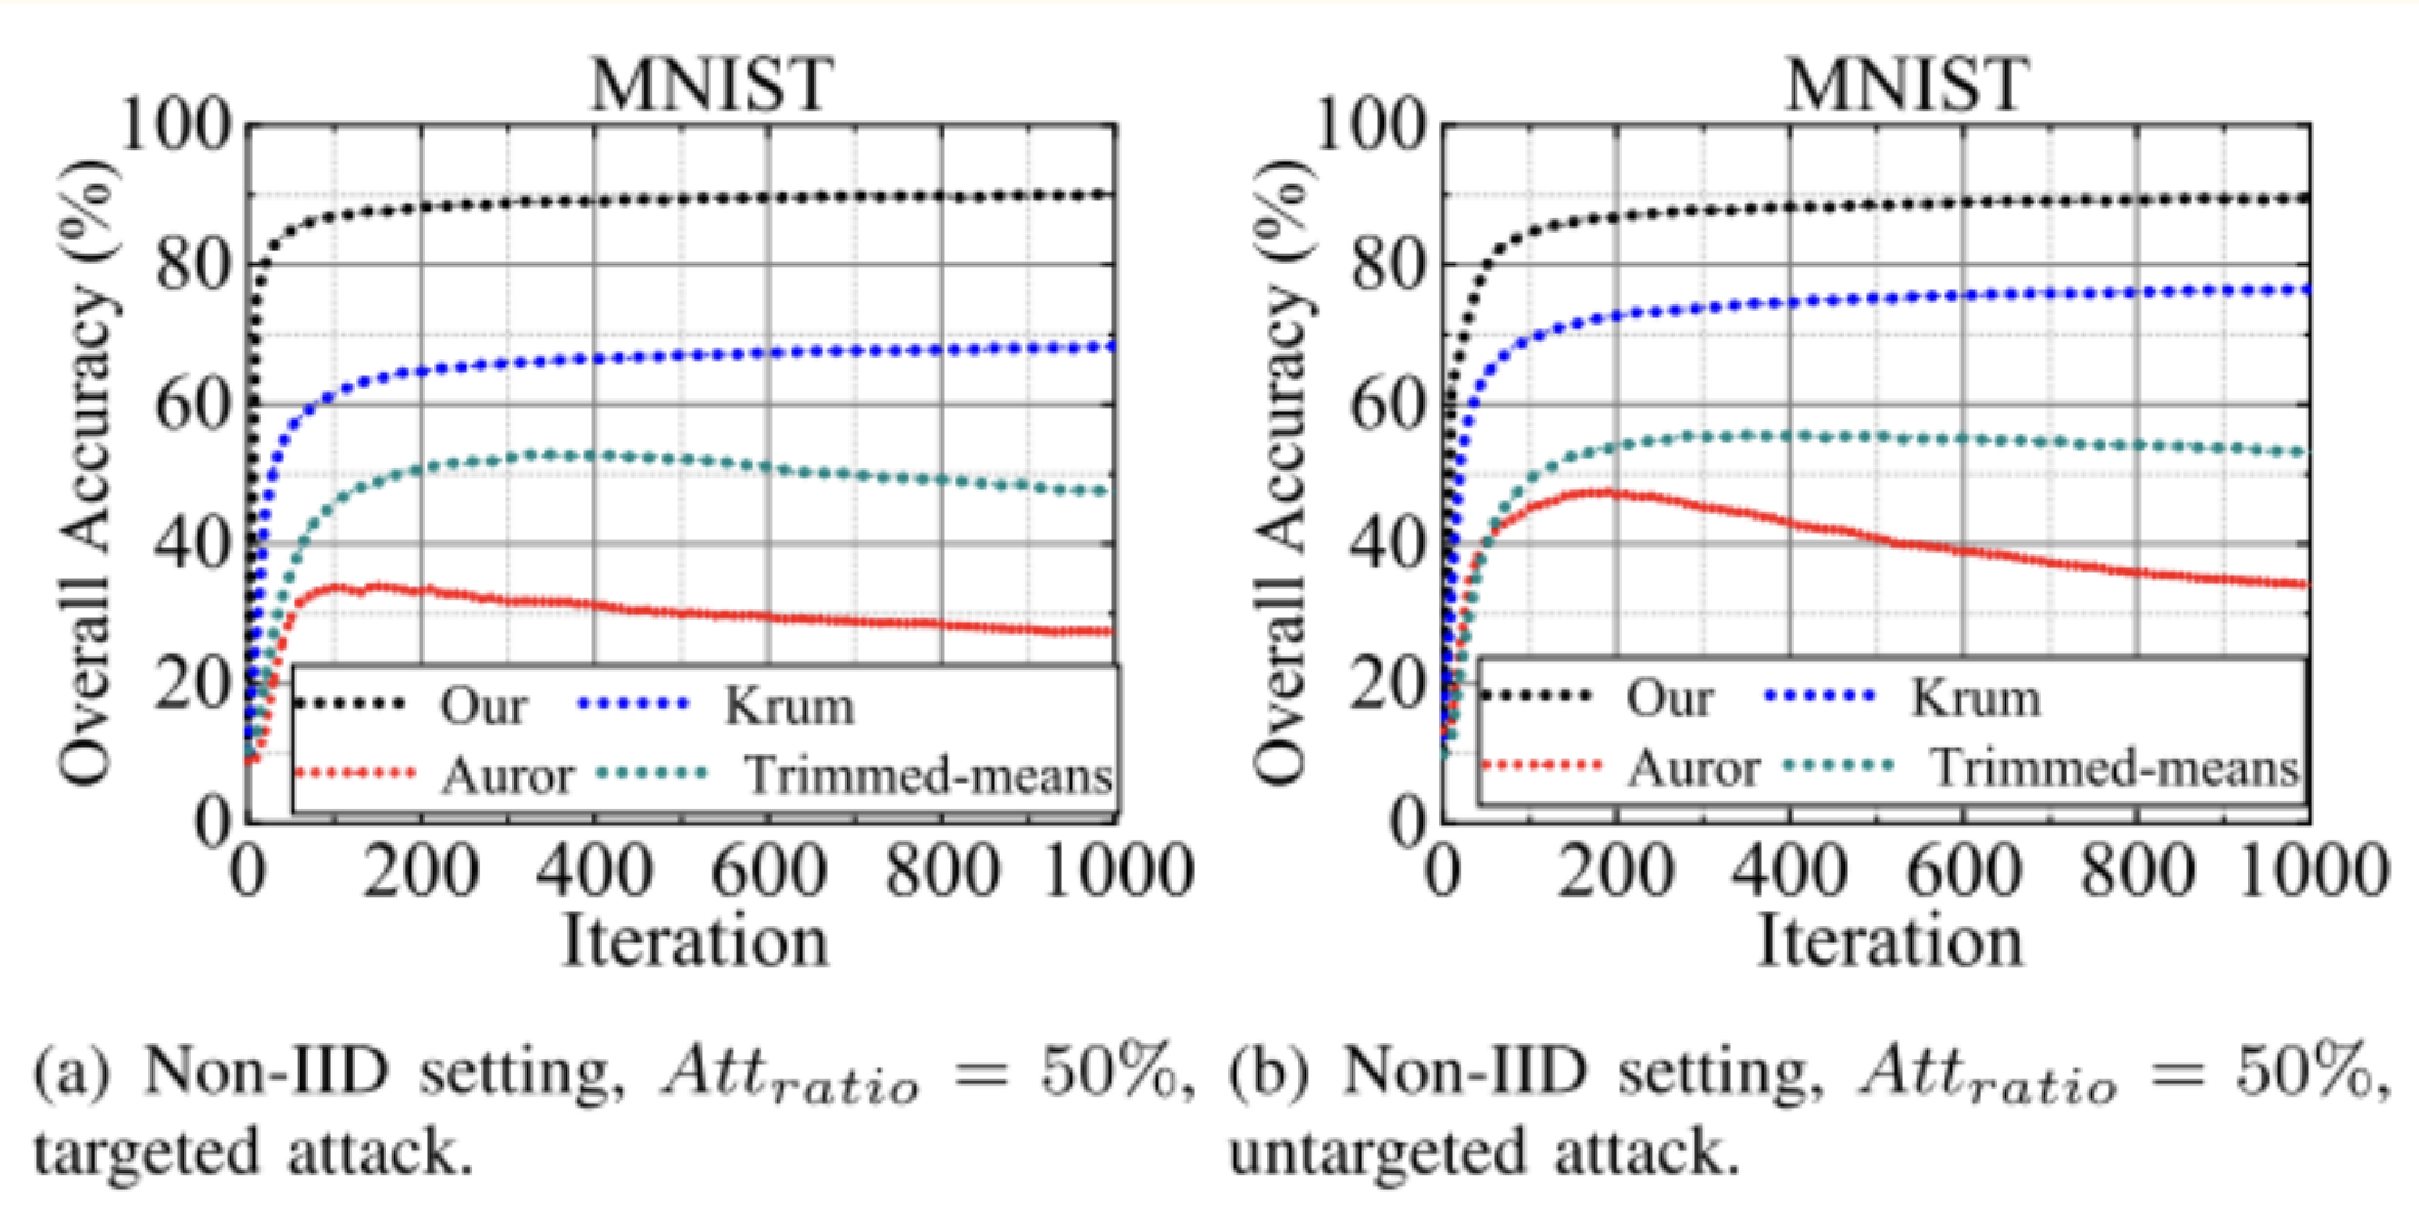
\includegraphics[width=0.8\linewidth]{resources/mnist-accuracy-comparison.pdf}
  \caption{MNIST accuracy comparison}
  \label{fig:mnsist-accuracy-comparison}
  %\vspace{-5mm}
\end{figure}

Finally, \Cref{fig:shield-fl-performance-with-iid-data} presents ShieldFL performance with IID data when the malicious users ratio is $50\%$.
The red dotted line presents the accuracy of the model without any attacks, while the greenish line shows the accuracy when the attack is performed without the involvement of ShieldFl.
Finally, the black line depicts the overall accuracy when ShieldFL was deployed, where it shows a high level of competency in identifying and eliminating the attack.
In the targeted attack, the ASR is around $11\%$, however, in the untargeted attack, the ASR is almost zero, which demonstrates that the attack was totally eliminated.

\begin{figure}[thb]
\centering
  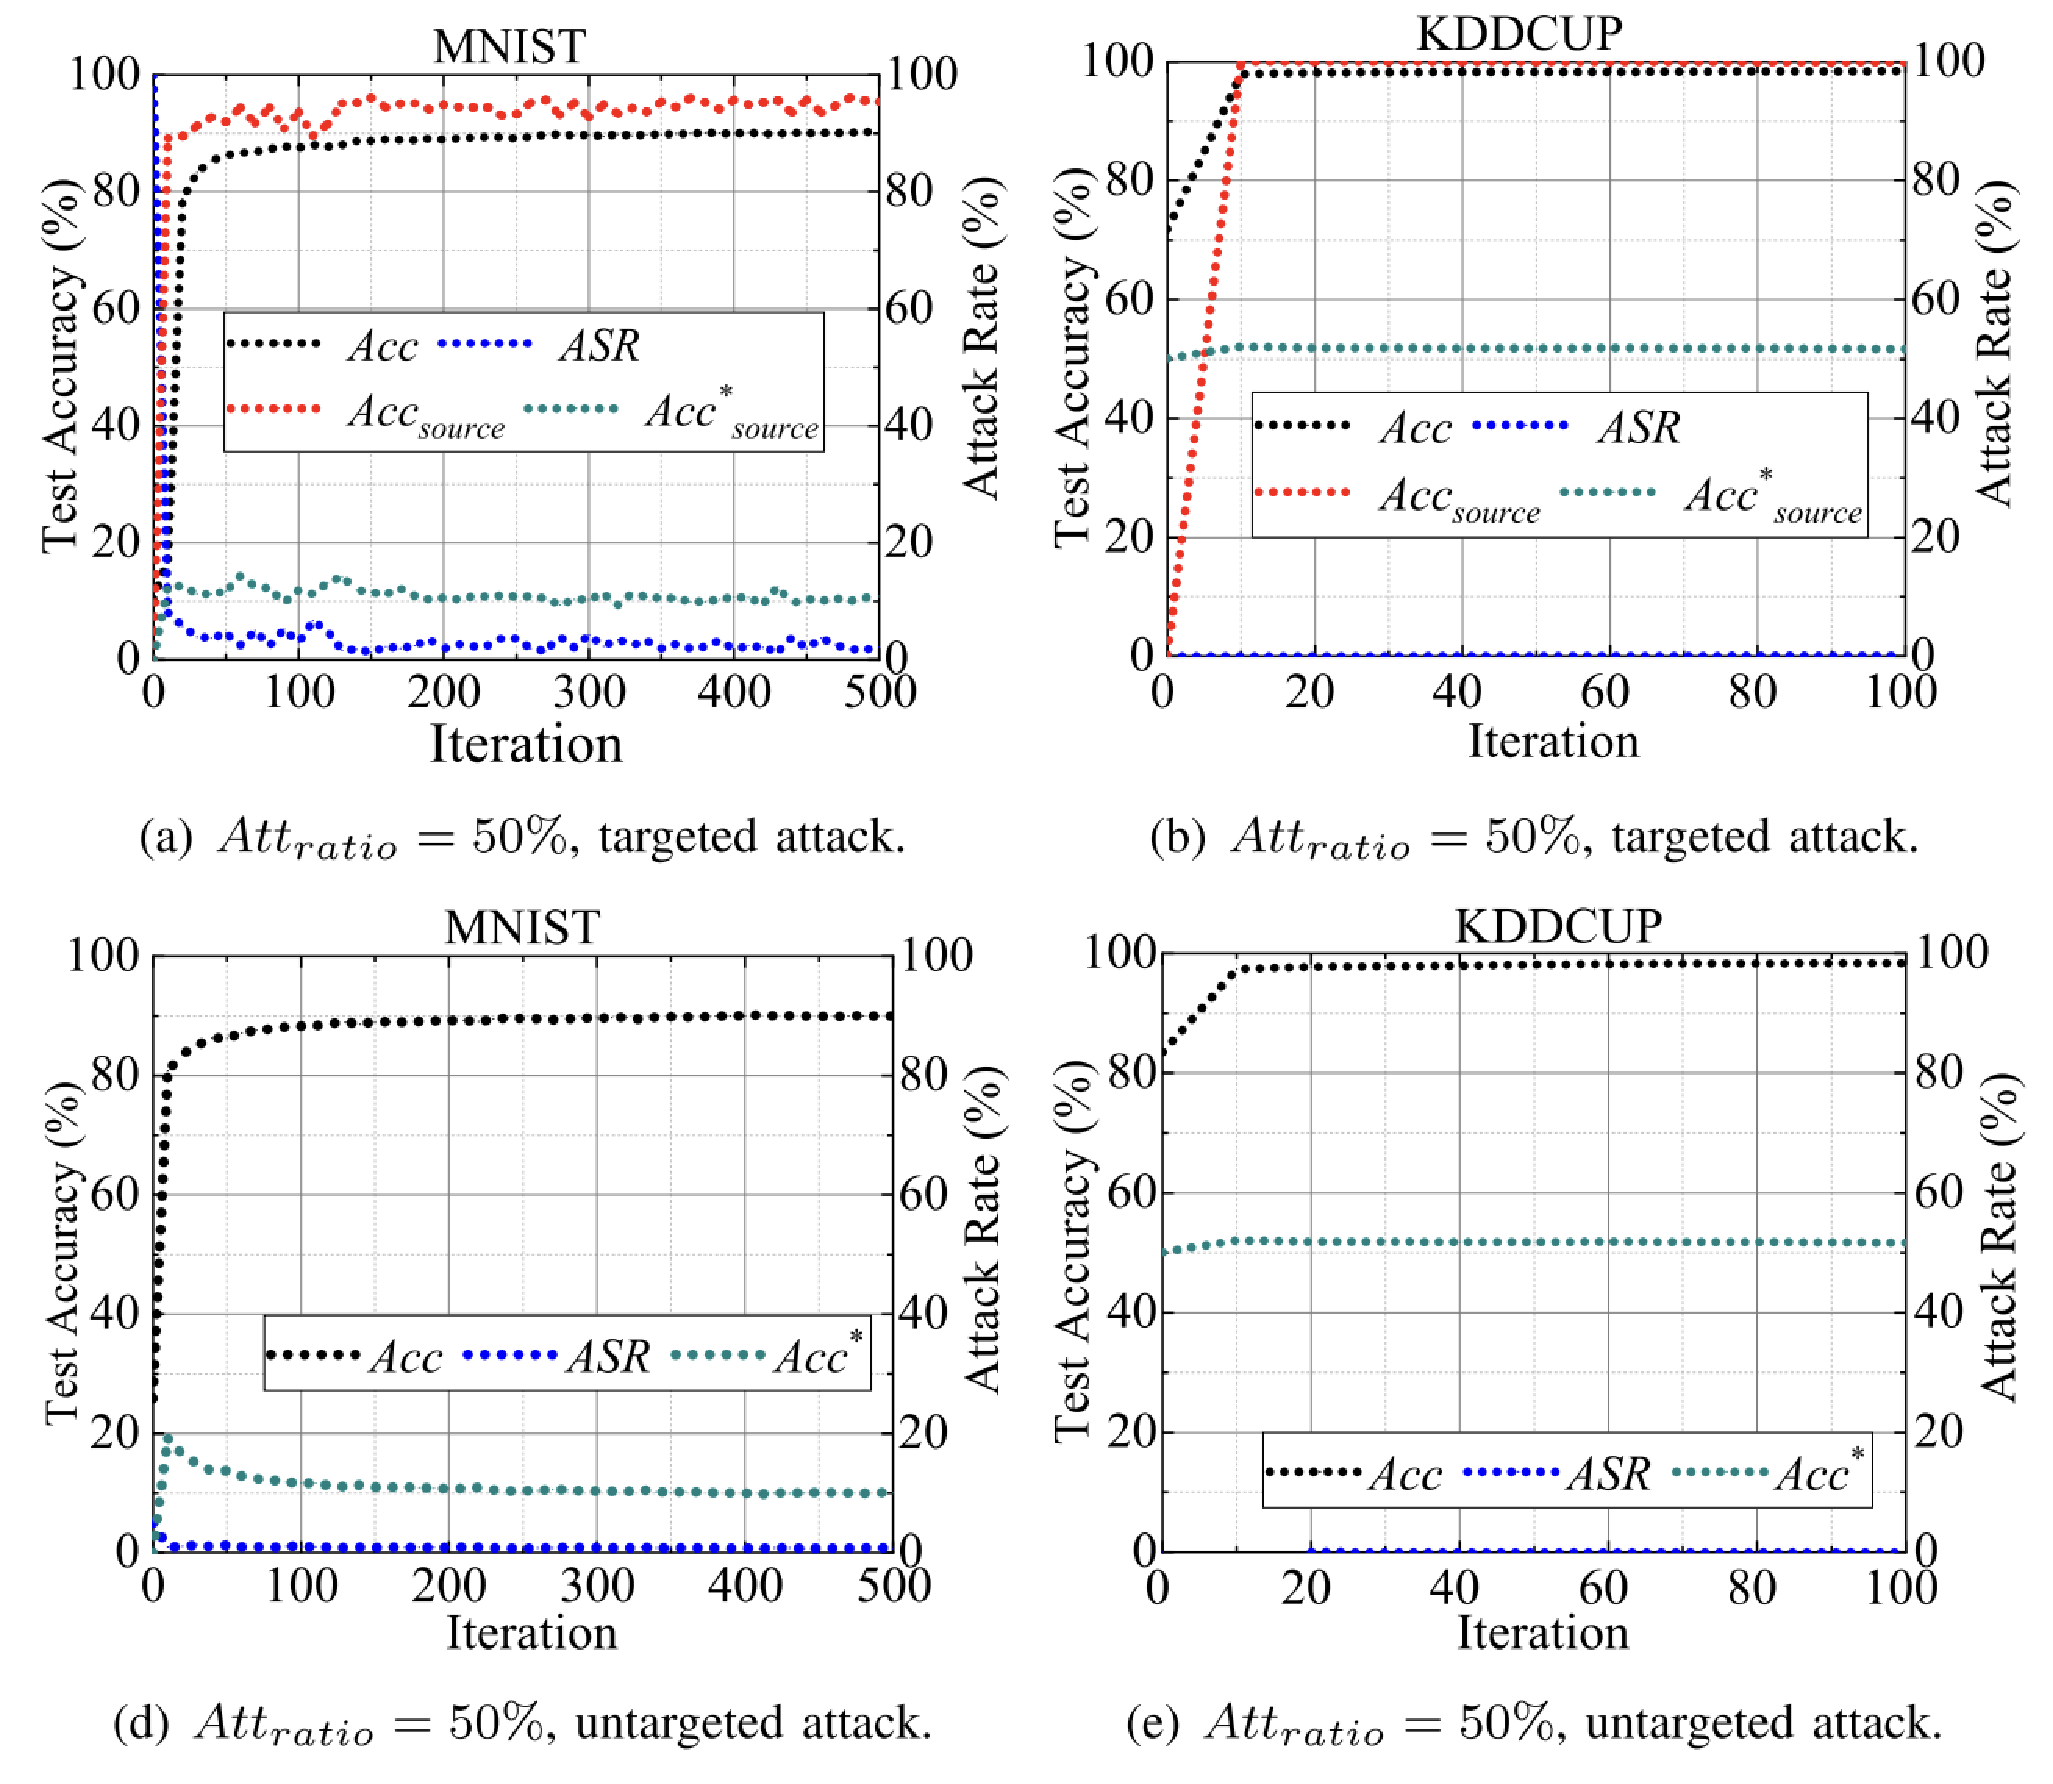
\includegraphics[width=0.8\linewidth]{resources/shield-fl-performance-with-iid-data.pdf}
  \caption{ShieldFL performance with IID data in MNIST and KDDCUP datasets}
  \label{fig:shield-fl-performance-with-iid-data}
  %\vspace{-5mm}
\end{figure}